\documentclass{standalone}
\usepackage{tikz}
\begin{document}
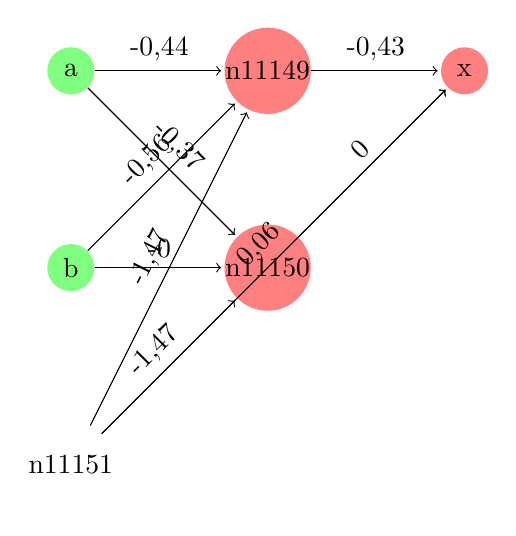
\begin{tikzpicture}[shorten >=1pt,->,draw=black!,node distance=2.5cm]
\tikzstyle{neuron}=[circle,fill=black!25,minimum size=17pt,inner sep=0pt]
\tikzstyle{constant}=[neuron, fill=white!50];
\tikzstyle{sigmoid}=[neuron, fill=red!50];
\tikzstyle{identity}=[neuron, fill=green!50];
\node [identity] (a) {a};
\node [identity,below of=a] (b) {b};
\node [constant,below of=b] (n11151) {n11151};
\node [sigmoid,right of=a] (n11149) {n11149};
\node [sigmoid,below of=n11149] (n11150) {n11150};
\node [sigmoid,right of=n11149] (x) {x};
\path[every node/.style={sloped,anchor=south,auto=false}]
(n11151) edge node {0,06} (x)
(n11151) edge node {-1,47} (n11150)
(n11151) edge node {-1,47} (n11149)
(b) edge node {-0,56} (n11149)
(b) edge node {-0} (n11150)
(a) edge node {-0,44} (n11149)
(a) edge node {-0,37} (n11150)
(n11149) edge node {-0,43} (x)
(n11150) edge node {0} (x)
;\end{tikzpicture}
\end{document}